% Options for packages loaded elsewhere
\PassOptionsToPackage{unicode}{hyperref}
\PassOptionsToPackage{hyphens}{url}
\PassOptionsToPackage{dvipsnames,svgnames,x11names}{xcolor}
%
\documentclass[
  a4paper,showtrims,openright,hidelinks]{oblivoir}

\usepackage{amsmath,amssymb}
\usepackage{iftex}
\ifPDFTeX
  \usepackage[T1]{fontenc}
  \usepackage[utf8]{inputenc}
  \usepackage{textcomp} % provide euro and other symbols
\else % if luatex or xetex
  \usepackage{unicode-math}
  \defaultfontfeatures{Scale=MatchLowercase}
  \defaultfontfeatures[\rmfamily]{Ligatures=TeX,Scale=1}
\fi
\usepackage{lmodern}
\ifPDFTeX\else  
    % xetex/luatex font selection
\fi
% Use upquote if available, for straight quotes in verbatim environments
\IfFileExists{upquote.sty}{\usepackage{upquote}}{}
\IfFileExists{microtype.sty}{% use microtype if available
  \usepackage[]{microtype}
  \UseMicrotypeSet[protrusion]{basicmath} % disable protrusion for tt fonts
}{}
\makeatletter
\@ifundefined{KOMAClassName}{% if non-KOMA class
  \IfFileExists{parskip.sty}{%
    \usepackage{parskip}
  }{% else
    \setlength{\parindent}{0pt}
    \setlength{\parskip}{6pt plus 2pt minus 1pt}}
}{% if KOMA class
  \KOMAoptions{parskip=half}}
\makeatother
\usepackage{xcolor}
\setlength{\emergencystretch}{3em} % prevent overfull lines
\setcounter{secnumdepth}{5}
% Make \paragraph and \subparagraph free-standing
\ifx\paragraph\undefined\else
  \let\oldparagraph\paragraph
  \renewcommand{\paragraph}[1]{\oldparagraph{#1}\mbox{}}
\fi
\ifx\subparagraph\undefined\else
  \let\oldsubparagraph\subparagraph
  \renewcommand{\subparagraph}[1]{\oldsubparagraph{#1}\mbox{}}
\fi

\usepackage{color}
\usepackage{fancyvrb}
\newcommand{\VerbBar}{|}
\newcommand{\VERB}{\Verb[commandchars=\\\{\}]}
\DefineVerbatimEnvironment{Highlighting}{Verbatim}{commandchars=\\\{\}}
% Add ',fontsize=\small' for more characters per line
\usepackage{framed}
\definecolor{shadecolor}{RGB}{241,243,245}
\newenvironment{Shaded}{\begin{snugshade}}{\end{snugshade}}
\newcommand{\AlertTok}[1]{\textcolor[rgb]{0.68,0.00,0.00}{#1}}
\newcommand{\AnnotationTok}[1]{\textcolor[rgb]{0.37,0.37,0.37}{#1}}
\newcommand{\AttributeTok}[1]{\textcolor[rgb]{0.40,0.45,0.13}{#1}}
\newcommand{\BaseNTok}[1]{\textcolor[rgb]{0.68,0.00,0.00}{#1}}
\newcommand{\BuiltInTok}[1]{\textcolor[rgb]{0.00,0.23,0.31}{#1}}
\newcommand{\CharTok}[1]{\textcolor[rgb]{0.13,0.47,0.30}{#1}}
\newcommand{\CommentTok}[1]{\textcolor[rgb]{0.37,0.37,0.37}{#1}}
\newcommand{\CommentVarTok}[1]{\textcolor[rgb]{0.37,0.37,0.37}{\textit{#1}}}
\newcommand{\ConstantTok}[1]{\textcolor[rgb]{0.56,0.35,0.01}{#1}}
\newcommand{\ControlFlowTok}[1]{\textcolor[rgb]{0.00,0.23,0.31}{#1}}
\newcommand{\DataTypeTok}[1]{\textcolor[rgb]{0.68,0.00,0.00}{#1}}
\newcommand{\DecValTok}[1]{\textcolor[rgb]{0.68,0.00,0.00}{#1}}
\newcommand{\DocumentationTok}[1]{\textcolor[rgb]{0.37,0.37,0.37}{\textit{#1}}}
\newcommand{\ErrorTok}[1]{\textcolor[rgb]{0.68,0.00,0.00}{#1}}
\newcommand{\ExtensionTok}[1]{\textcolor[rgb]{0.00,0.23,0.31}{#1}}
\newcommand{\FloatTok}[1]{\textcolor[rgb]{0.68,0.00,0.00}{#1}}
\newcommand{\FunctionTok}[1]{\textcolor[rgb]{0.28,0.35,0.67}{#1}}
\newcommand{\ImportTok}[1]{\textcolor[rgb]{0.00,0.46,0.62}{#1}}
\newcommand{\InformationTok}[1]{\textcolor[rgb]{0.37,0.37,0.37}{#1}}
\newcommand{\KeywordTok}[1]{\textcolor[rgb]{0.00,0.23,0.31}{#1}}
\newcommand{\NormalTok}[1]{\textcolor[rgb]{0.00,0.23,0.31}{#1}}
\newcommand{\OperatorTok}[1]{\textcolor[rgb]{0.37,0.37,0.37}{#1}}
\newcommand{\OtherTok}[1]{\textcolor[rgb]{0.00,0.23,0.31}{#1}}
\newcommand{\PreprocessorTok}[1]{\textcolor[rgb]{0.68,0.00,0.00}{#1}}
\newcommand{\RegionMarkerTok}[1]{\textcolor[rgb]{0.00,0.23,0.31}{#1}}
\newcommand{\SpecialCharTok}[1]{\textcolor[rgb]{0.37,0.37,0.37}{#1}}
\newcommand{\SpecialStringTok}[1]{\textcolor[rgb]{0.13,0.47,0.30}{#1}}
\newcommand{\StringTok}[1]{\textcolor[rgb]{0.13,0.47,0.30}{#1}}
\newcommand{\VariableTok}[1]{\textcolor[rgb]{0.07,0.07,0.07}{#1}}
\newcommand{\VerbatimStringTok}[1]{\textcolor[rgb]{0.13,0.47,0.30}{#1}}
\newcommand{\WarningTok}[1]{\textcolor[rgb]{0.37,0.37,0.37}{\textit{#1}}}

\providecommand{\tightlist}{%
  \setlength{\itemsep}{0pt}\setlength{\parskip}{0pt}}\usepackage{longtable,booktabs,array}
\usepackage{calc} % for calculating minipage widths
% Correct order of tables after \paragraph or \subparagraph
\usepackage{etoolbox}
\makeatletter
\patchcmd\longtable{\par}{\if@noskipsec\mbox{}\fi\par}{}{}
\makeatother
% Allow footnotes in longtable head/foot
\IfFileExists{footnotehyper.sty}{\usepackage{footnotehyper}}{\usepackage{footnote}}
\makesavenoteenv{longtable}
\usepackage{graphicx}
\makeatletter
\def\maxwidth{\ifdim\Gin@nat@width>\linewidth\linewidth\else\Gin@nat@width\fi}
\def\maxheight{\ifdim\Gin@nat@height>\textheight\textheight\else\Gin@nat@height\fi}
\makeatother
% Scale images if necessary, so that they will not overflow the page
% margins by default, and it is still possible to overwrite the defaults
% using explicit options in \includegraphics[width, height, ...]{}
\setkeys{Gin}{width=\maxwidth,height=\maxheight,keepaspectratio}
% Set default figure placement to htbp
\makeatletter
\def\fps@figure{htbp}
\makeatother

%%%% fonts
%% 코드 overflow 방지
\usepackage{fvextra}
\DefineVerbatimEnvironment{Highlighting}{Verbatim}{breaklines,commandchars=\\\{\}}
\makeatletter
\makeatother
\makeatletter
\makeatother
\makeatletter
\@ifpackageloaded{caption}{}{\usepackage{caption}}
\AtBeginDocument{%
\ifdefined\contentsname
  \renewcommand*\contentsname{Table of contents}
\else
  \newcommand\contentsname{Table of contents}
\fi
\ifdefined\listfigurename
  \renewcommand*\listfigurename{List of Figures}
\else
  \newcommand\listfigurename{List of Figures}
\fi
\ifdefined\listtablename
  \renewcommand*\listtablename{List of Tables}
\else
  \newcommand\listtablename{List of Tables}
\fi
\ifdefined\figurename
  \renewcommand*\figurename{그림}
\else
  \newcommand\figurename{그림}
\fi
\ifdefined\tablename
  \renewcommand*\tablename{표}
\else
  \newcommand\tablename{표}
\fi
}
\@ifpackageloaded{float}{}{\usepackage{float}}
\floatstyle{ruled}
\@ifundefined{c@chapter}{\newfloat{codelisting}{h}{lop}}{\newfloat{codelisting}{h}{lop}[chapter]}
\floatname{codelisting}{Listing}
\newcommand*\listoflistings{\listof{codelisting}{List of Listings}}
\makeatother
\makeatletter
\@ifpackageloaded{caption}{}{\usepackage{caption}}
\@ifpackageloaded{subcaption}{}{\usepackage{subcaption}}
\makeatother
\makeatletter
\makeatother
\ifLuaTeX
  \usepackage{selnolig}  % disable illegal ligatures
\fi
\usepackage[]{biblatex}
\addbibresource{references.bib}
\IfFileExists{bookmark.sty}{\usepackage{bookmark}}{\usepackage{hyperref}}
\IfFileExists{xurl.sty}{\usepackage{xurl}}{} % add URL line breaks if available
\urlstyle{same} % disable monospaced font for URLs
\hypersetup{
  pdftitle={지리정보시스템과 프롭테크: 도구의 진화와 미래 방향},
  colorlinks=true,
  linkcolor={blue},
  filecolor={Maroon},
  citecolor={Blue},
  urlcolor={Blue},
  pdfcreator={LaTeX via pandoc}}

\title{지리정보시스템과 프롭테크: 도구의 진화와 미래 방향}
\author{이광춘\textsuperscript{1,*}}
\date{2023-09-01}

\begin{document}
\maketitle
\begin{abstract}
오픈소스 소프트웨어와 공간정보 공공데이터가 넘쳐나고 있는 가운데, 시민
데이터 과학자의 중요성이 증가하고 있다. 그러나, 지난 50년 동안 빠르게
발전해 온 지리 정보 시스템(GIS) 분야를 부동산 기술(프롭테크) 관점에서
바라보면 가속되고 있는 도구의 발전이 가져올 미래 방향을 유추할 수 있다.
다른 과학 및 엔지니어링 분야에서와 마찬가지로, GIS 분야 또한 지속적인
도구의 발전을 통해 큰 혁신이 일어나고 있다. 본 연구에서는 GIS 도구의
발전 과정을 살펴보고, 사례로 제시된 코드와 코드를 지탱하는 도구를 코드
뒤에 숨겨진 기술 생태계를 이해하고 프롭테크 미래발전 방향을 함께
가늠하고자 한다.
\end{abstract}
\textsuperscript{1} 한국 R 사용자회, 서울, 대한민국

\textsuperscript{*} Correspondence:
\href{mailto:victor@r2bit.com}{이광춘
\textless{}victor@r2bit.com\textgreater{}}

\hypertarget{uxb4e4uxc5b4uxac00uxba70}{%
\section{들어가며}\label{uxb4e4uxc5b4uxac00uxba70}}

최근 OpenAI사가 공개한 챗GPT는 인공지능 분야 자체도 큰 반향을 일으키고
있지만, 다른 분야에도 커다란 변화를 일으키고 있는데 가장 큰 이유는
쓸만한 도구가 마련되었기 때문이다. 시대에 맞는 적절한 도구 없이
지리정보시스템과 프롭테크를 지향하는 것은 커다란 모순이기 때문에
지리학에 대한 주요 개념을 먼저 살펴본 후에 도구의 진화를 살펴보고 진화된
도구를 통한 사례로 프롭테크의 미래를 함께 조망해보자.
\autocite{ChatGPT2023}

지리학(Geography)은 가장 오래된 과학 중 하나로 꼽히며, 학생때부터 교실
여기저기에서 볼 수 있는 지도가 아마도 처음 접한 데이터 시각화 산출물일
것이다. 지리학은 지구의 곡률을 정확히 파악하여 지구의 크기와 모양,
중력에 대한 이해를 높이는 데 중요한 역할을 수행했을 뿐만 아니라 대항해
시대 지도가 매우 큰 기여를 했고, 현대에 와서 지리학 데이터 응용 범위는
더욱 확장되어, 민간과 국방 범위를 가리지 않고 상업적으로 입점위치 선정,
우주 탐사, 군사 작전, 인구이동 패턴 분석 등 다방면에서 요긴한 역할을
수행하고 있다. \textbf{지리정보시스템(GIS)}은 공간 위치를 분석하고
정보를 지도와 필요한 경우 3D로 시각화하여 데이터 패턴, 관계, 상황 등에
대한 심도 깊은 이해를 제공하여 의사결정을 지원한다.

먼저 좌표계를 살펴보자. 지도 자체가 불가피하게 왜곡된 현실을 시각적으로
표현하기 때문에 `현실의 축소판'(Maps are scale models of reality)이라고
할 수 있다. 예를 들어, 사과 껍질을 벗겨 펼친 것처럼, 평면화시켜 지도를
제작한다. 특히, \textbf{지리 좌표계(Geographic Coordinate System)}와
\textbf{투영 좌표계(Projected Coordinate System)}는 지도 작성과 공간
분석에서 중요한 개념이다. 간단히 요약하면, 지리 좌표계는 정확한 위치
정보를 제공하는 반면, 투영 좌표계는 거리와 면적 측정에 더 적합하다. 지리
좌표계는 지구상 위치를 설명하며, 지구가 둥글기 때문에 주로 각도 단위로
측정되고, 기준점에 상관없이 위치가 달라지지 않으므로 절대 좌표계다. 투영
좌표계는 지리 좌표계를 평면화한 것으로, 투영 좌표계를 사용할 경우 직선을
이용해 거리를 측정할 수 있어, 토지 이용 계획, 건물 배치, 거리 측정
등에서 유용하다. \autocite{lovelace2019geocomputation}

다음으로 지도학의 대표적인 파일 형식을 살펴보자.
\textbf{지도학(Cartography)}은 지도를 작성하는 중요한 실무분야로 과거
벡터 데이터 형식으로 대표적인 \texttt{Shapefile} 파일을 통해 점, 다각형,
선으로 지리적 정보를 표현했다면, GIS 분야에 오픈소스 소프트웨어 문화가
확산되면서 \texttt{Geopackage}, \texttt{GeoJSON}, \texttt{KML}과 같은
다른 파일형식도 인기를 얻고 있다. GIS 데이터는 지도 뿐만 아니라 R 혹은
파이썬 프로그래밍 언어를 활용하여 다른 형태의 (비)정형 데이터와 결합한
교차분석이 일반화되고 있다.

전통적인 \textbf{벡터(Vector)} \texttt{Shapefile} 파일과 함께
\textbf{래스터(Raster)} 데이터는 GIS에서 큰 축을 담당하는 대표적인
데이터 형식이다. 벡터 데이터가 점, 선, 다각형 등의 기하학적 형태로 주로
경계선, 위치 정보 등을 정확하게 표현할 때 사용되는 반면, 래스터 데이터는
픽셀이나 셀 배열로 정보를 표현한다는 점에서 차이가 난다. 각 픽셀은
고유값을 가지며, 색상, 높이, 밀도 등 다양한 형태 정보를 표현하는데
용이하다.

GIS에서 계층(레이어, Layer)별로 나눠 데이터를 표현하고, 이를 결합하여
공간정보 지도형태 산출물을 얻는다. 한 구획의 토지(parcle), 공간 정보를
점, 선, 다각형 같은 벡터 데이터로 표현하고 비공간 정보는 소유권, 토지
이용, 구역 분류, 평가 가치 등 다양한 속성(칼럼) 데이터프레임과 결합하여
작업한다. Figure~\ref{fig-layers} 에 실제 세상이 벡터와 래스터 데이터로
표현하는 사례가 제시되어 있다.

\begin{figure}

{\centering 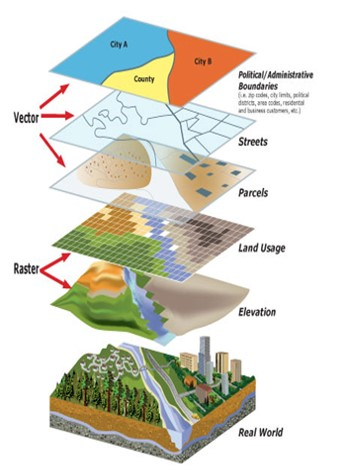
\includegraphics{images/gis_layers.jpg}

}

\caption{\label{fig-layers}GIS 벡터와 래스터 계층, 출처:
http://gis.sbcounty.gov/}

\end{figure}

\hypertarget{uxb3c4uxad6cuxc758-uxc9c4uxd654}{%
\section{도구의 진화}\label{uxb3c4uxad6cuxc758-uxc9c4uxd654}}

GIS, 좌표계, 파일 형식, 계층(Layer), 교차분석 등 주요개념을 바탕으로
도구 진화과정을 살펴보자. 초기 PC가 보급되면서 1980년대 GIS 시스템은
사일로 형태 고가 시스템이었으며, 1990년대에는 1980년대 개발된 GIS
시스템간 연결이 시작되면서 스파게티 현상이 심해지면서 새로운
애플리케이션과 파일 형식이 도입되는데 필요 이상의 낭비가 심해지는 구조가
되었다.

2000년대 GDAL(Geospatial Data Abstraction Layer)이 등장하여 개발자가 각
파일 형식별로 서로 다른 드라이버를 작성하는 대신 GDAL 클라이언트
드라이버만 개발하면 되기 때문에 일대 혁신이 일어났다. 2010년대는
인공위성을 통한 대량의 데이터가 넘쳐나며 이를 저장하기 위해서 클라우드
서비스가 우후죽순처럼 생겨났고 각기 다른 파편화된 진화과정이 일어났다.
2020년대 넘어서면서 1990년대와 유사한 상황이 재현되었고, 이를 해결하고
새로운 전환점을 만들기 위해 \texttt{OpenEO}가 제시되며 사용자와 데이터
센터 사이에서 새로운 표준으로 자리잡게 되면서 R, 파이썬 등 데이터 과학
프로그래밍 언어를 통한 공간정보 가치 창출이 용이해졌다.
\autocite{Pebesma2016}

\begin{figure}

{\centering 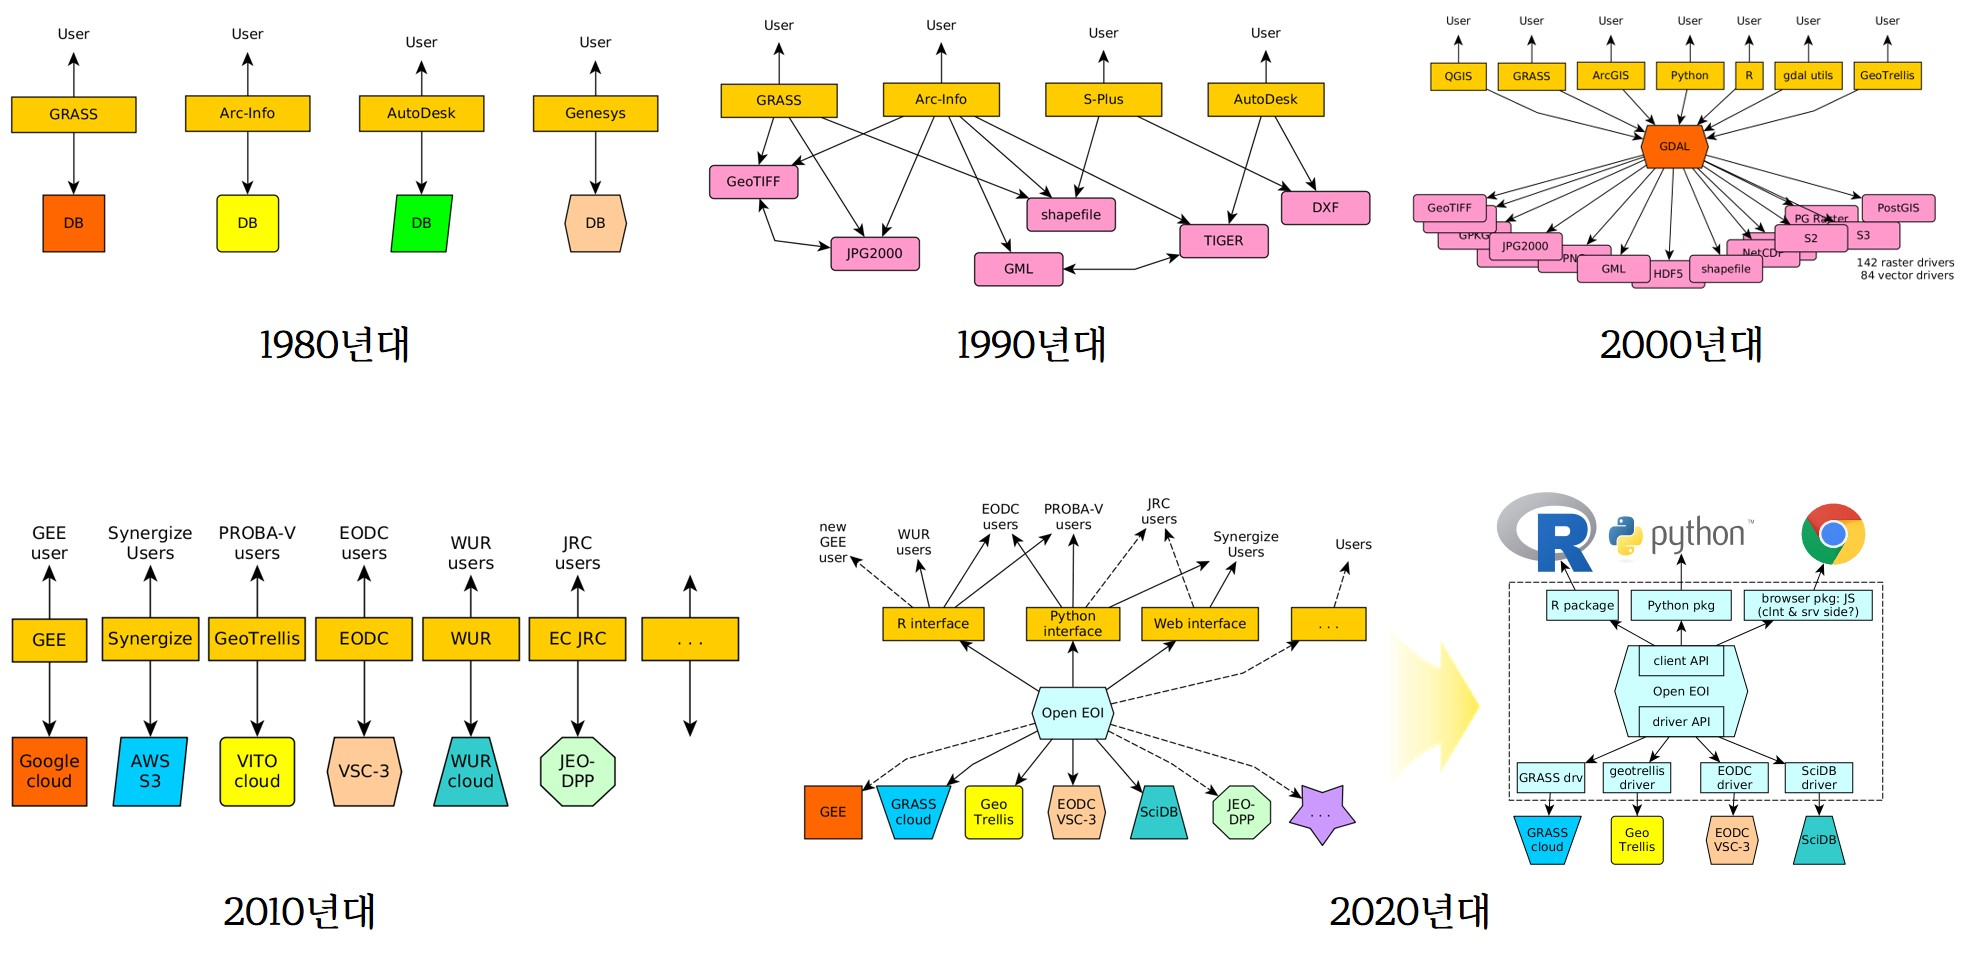
\includegraphics{images/gis_evolution.jpg}

}

\caption{GIS 도구 진화과정}

\end{figure}

\hypertarget{gis-uxc0dduxd0dcuxacc4}{%
\section{GIS 생태계}\label{gis-uxc0dduxd0dcuxacc4}}

인간은 오랜 역사 동안 다양한 도구를 개발하고 사용해 왔으며, GIS에서도
도구는 단순한 계산부터 복잡한 데이터 분석, 시각화를 통한 의사결정지원,
최근 거대언어모형(LLM) 인공지능까지 다양한 형태로 기여하고 있다.

현재 직면한 문제를 해결하는데 과거 도구를 사용하는 것은 마치 철기시대에
석기시대 도구를 사용하는 것과 다름이 없다. 따라서, 데이터를 통해 가치를
만드는 데이터 과학자 입장에서 도구의 선택은 매우 중요할 수 밖에 없다.

\begin{figure}

{\centering 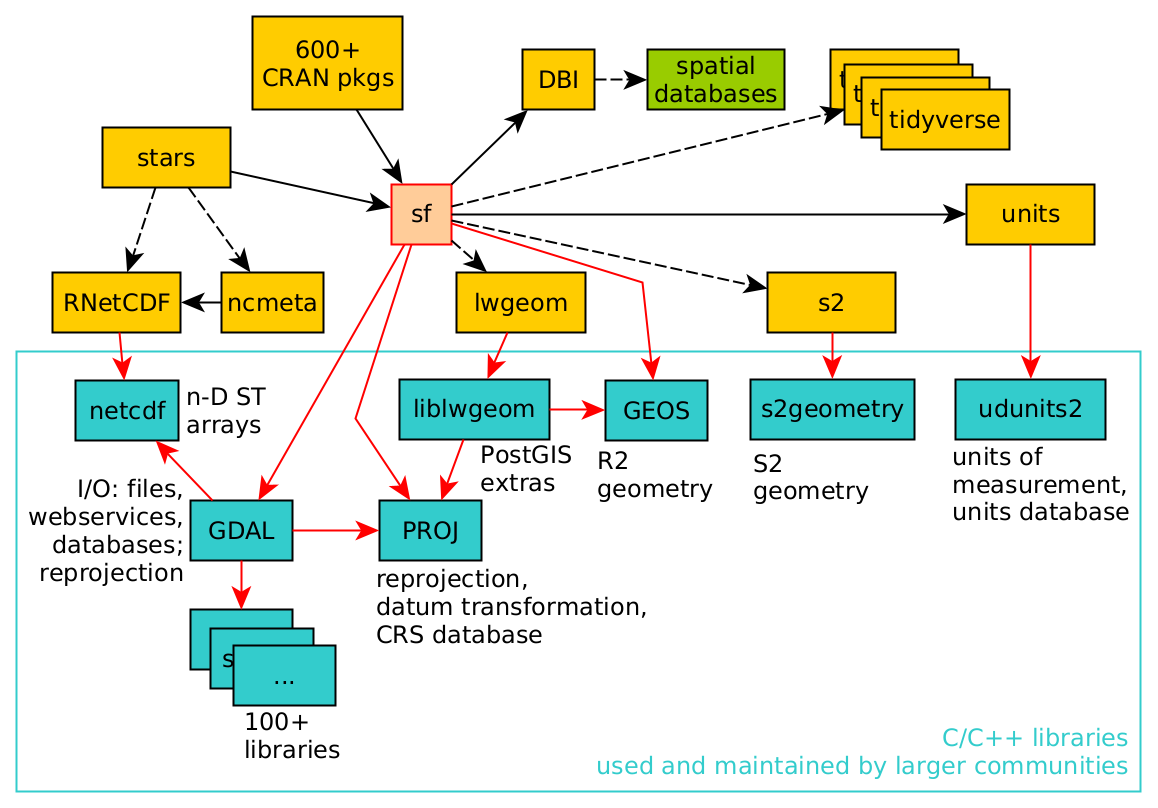
\includegraphics{images/sf_deps.png}

}

\caption{\label{fig-evolution}\texttt{sf} 패키지와 의존성 - 화살표는
강한 의존성, 점선 화살표는 약한 의존성}

\end{figure}

현재 R 공간정보 생태계는 공간정보 도구 진화과정을 몇차례 경험한 후에
Figure~\ref{fig-evolution} 처럼 자리를 잡았다. 결론부터 들어가면
\texttt{sf} 패키지가 생태계의 중심으로 자리 잡았으며, 사용자와 개발자는
\texttt{sf} 패키지를 통해 상당수 공간정보 데이터 문제를 해결할 수 있게
되었다. 하지만, \texttt{sf} 패키지는 C/C++ 라이브러리에 크게 의존성하기
때문에 각 라이브러리를 살펴보는 것은 향후 GIS 개발자와 분석가로 현업에서
활약하는데 큰 도움이 될 것으로 보인다.

\texttt{GDAL}, \texttt{GEOS}, \texttt{PROJ}, \texttt{liblwgeom},
\texttt{s2geometry}, \texttt{NetCDF}, \texttt{udunits2}는 C/C++
라이브러리를 개발, 유지보수, 지원하는 커뮤니티가 존재하는 반면 R,
파이썬, 줄리아(Julia), 자바스크립트는 대화형 인터페이스를 통해
라이브러리를 활용하는 커뮤니티도 존재한다. \autocite{sds}

\begin{itemize}
\tightlist
\item
  \texttt{GDAL} (Geospatial Data Abstraction Library) 라이브러리는 공간
  데이터 처리에 있어 멀티툴의 대명사인 스위스군 칼(SAK, Swiss Army
  Knife)이라는 별명을 갖고 있고 100개가 넘는 다른 라이브러리와 연결되어
  다양한 공간 데이터를 불러오고, 처리하고, 내보내는 기능을 제공한다.
\item
  \texttt{PROJ}는 지도 투영 및 데이터 변환을 위한 라이브러리로, 하나의
  좌표계에서 다른 좌표계로 좌표를 변환할 때 유용하다.
\item
  \texttt{GEOS} (Geometry Engine Open Source)와 \texttt{s2geometry}
  라이브러리는 기하학 연산에 사용하며, 길이, 면적, 거리를 측정하거나
  연산작업에 사용되며 \(R^2\)로 표기되며 \texttt{GEOS}는 평평한 2차원
  공간에, \(S^2\)로 표기되며 \texttt{s2geometry}는 구형 공간에 사용한다.
\item
  \texttt{NetCDF}는 파일 형식이며 C 라이브러리로, 어떤 차원 배열도
  정의할 수 있으며 특히 (기후) 모형개발 커뮤니티에서 널리 사용된다.
  \texttt{Udunits2}는 측정 단위의 데이터베이스 및 소프트웨어
  라이브러리로, 단위의 변환과 파생 단위, 사용자 정의 단위를 처리한다.
  \texttt{liblwgeom}은 PostGIS 구성 요소로, \texttt{GDAL},
  \texttt{GEOS}에서 누락된 몇 가지 루틴을 포함한다.
  \autocite{Pebesma2016}
\end{itemize}

\hypertarget{uxc0acuxb840}{%
\section{사례}\label{uxc0acuxb840}}

\texttt{sf} 패키지가 추상화된 함수를 제공하기 때문에 R 공간정보
생태계에서 \texttt{GDAL} 라이브러리를 GIS 분석가가 직접적으로 다룰 일은
없다. 하지만, GIS 도구를 활용하여 2023년 7월 기준 시도별 인구수를
대한민국 지도위에 도식화하기 위해서는 R 공간정보 생태계를 구성하는
다양한 도구가 꼭 필요하다. 먼저, 지도 데이터를 다루기 위해 \texttt{sf}
패키지를 사용하고 통계청(KOSIS) 데이터를 처리하기 위해
\texttt{tidyverse} 패키지 도구를 활용하고 오픈지도 개발자가 공개한
\texttt{geojson} 파일을 결합하여 인구수를 시도 수준에서 시도별 인구수
색상을 달리하여 지도위에 시각화한다. 작성된 코드는 R로 작성되었지만
파이썬 진영에도 공간정보 생태계도 유사한 도구가 준비되어 있어 각자
사용하기 좋은 도구를 가지고 의미있는 결과물을 만들어내고
있다.\autocite{wickham2019welcome}

\begin{Shaded}
\begin{Highlighting}[]
\FunctionTok{library}\NormalTok{(sf)}
\FunctionTok{library}\NormalTok{(tidyverse)}
\FunctionTok{sf\_use\_s2}\NormalTok{(}\ConstantTok{FALSE}\NormalTok{)}

\DocumentationTok{\#\# 지도}
\NormalTok{korea\_map }\OtherTok{\textless{}{-}} \FunctionTok{read\_sf}\NormalTok{(}\StringTok{"data/HangJeongDong\_ver20230401.geojson"}\NormalTok{)}

\NormalTok{sido\_map }\OtherTok{\textless{}{-}}\NormalTok{ korea\_map }\SpecialCharTok{|\textgreater{}} 
  \FunctionTok{group\_by}\NormalTok{(sidonm) }\SpecialCharTok{|\textgreater{}} 
  \FunctionTok{summarise}\NormalTok{(}\AttributeTok{geometry =}\NormalTok{ sf}\SpecialCharTok{::}\FunctionTok{st\_union}\NormalTok{(geometry))}

\DocumentationTok{\#\# 23년 7월 인구수(KOSIS) 행정구역별, 성별 인구수}
\NormalTok{pop\_tbl }\OtherTok{\textless{}{-}} \FunctionTok{read\_csv}\NormalTok{(}\StringTok{"data/행정구역\_시군구\_별\_\_성별\_인구수\_20230831223248.csv"}\NormalTok{,}
         \AttributeTok{locale=}\FunctionTok{locale}\NormalTok{(}\AttributeTok{encoding=}\StringTok{"euc{-}kr"}\NormalTok{), }\AttributeTok{skip =} \DecValTok{1}\NormalTok{) }\SpecialCharTok{|\textgreater{}} 
  \FunctionTok{set\_names}\NormalTok{(}\FunctionTok{c}\NormalTok{(}\StringTok{"sidonm"}\NormalTok{, }\StringTok{"인구수"}\NormalTok{)) }\SpecialCharTok{|\textgreater{}} 
  \FunctionTok{mutate}\NormalTok{(}\AttributeTok{sidonm =} \FunctionTok{if\_else}\NormalTok{(sidonm }\SpecialCharTok{==} \StringTok{"강원특별자치도"}\NormalTok{, }\StringTok{"강원도"}\NormalTok{, sidonm))}

\NormalTok{sigo\_gg }\OtherTok{\textless{}{-}}\NormalTok{ sido\_map }\SpecialCharTok{|\textgreater{}} 
  \FunctionTok{left\_join}\NormalTok{(pop\_tbl) }\SpecialCharTok{|\textgreater{}} 
  \FunctionTok{ggplot}\NormalTok{() }\SpecialCharTok{+}
    \FunctionTok{geom\_sf}\NormalTok{(}\FunctionTok{aes}\NormalTok{(}\AttributeTok{geometry =}\NormalTok{ geometry, }\AttributeTok{fill =} \FunctionTok{cut}\NormalTok{(인구수, }\DecValTok{10}\NormalTok{)), }\AttributeTok{show.legend =} \ConstantTok{FALSE}\NormalTok{) }\SpecialCharTok{+}
\NormalTok{    ggrepel}\SpecialCharTok{::}\FunctionTok{geom\_label\_repel}\NormalTok{(}\FunctionTok{aes}\NormalTok{(}\AttributeTok{label =}\NormalTok{ sidonm, }\AttributeTok{geometry =}\NormalTok{ geometry), }
                              \AttributeTok{size =} \DecValTok{3}\NormalTok{, }\AttributeTok{stat =} \StringTok{"sf\_coordinates"}\NormalTok{) }\SpecialCharTok{+}
    \FunctionTok{theme\_void}\NormalTok{() }\SpecialCharTok{+}
    \FunctionTok{scale\_fill\_brewer}\NormalTok{(}\AttributeTok{palette =} \StringTok{"OrRd"}\NormalTok{)}

\NormalTok{ragg}\SpecialCharTok{::}\FunctionTok{agg\_jpeg}\NormalTok{(}\StringTok{"images/GIS\_tools.jpeg"}\NormalTok{,}
               \AttributeTok{width =} \DecValTok{10}\NormalTok{, }\AttributeTok{height =} \DecValTok{7}\NormalTok{, }\AttributeTok{units =} \StringTok{"in"}\NormalTok{, }\AttributeTok{res =} \DecValTok{600}\NormalTok{)}
\NormalTok{sigo\_gg}
\FunctionTok{dev.off}\NormalTok{()}
\end{Highlighting}
\end{Shaded}

\begin{figure}

{\centering 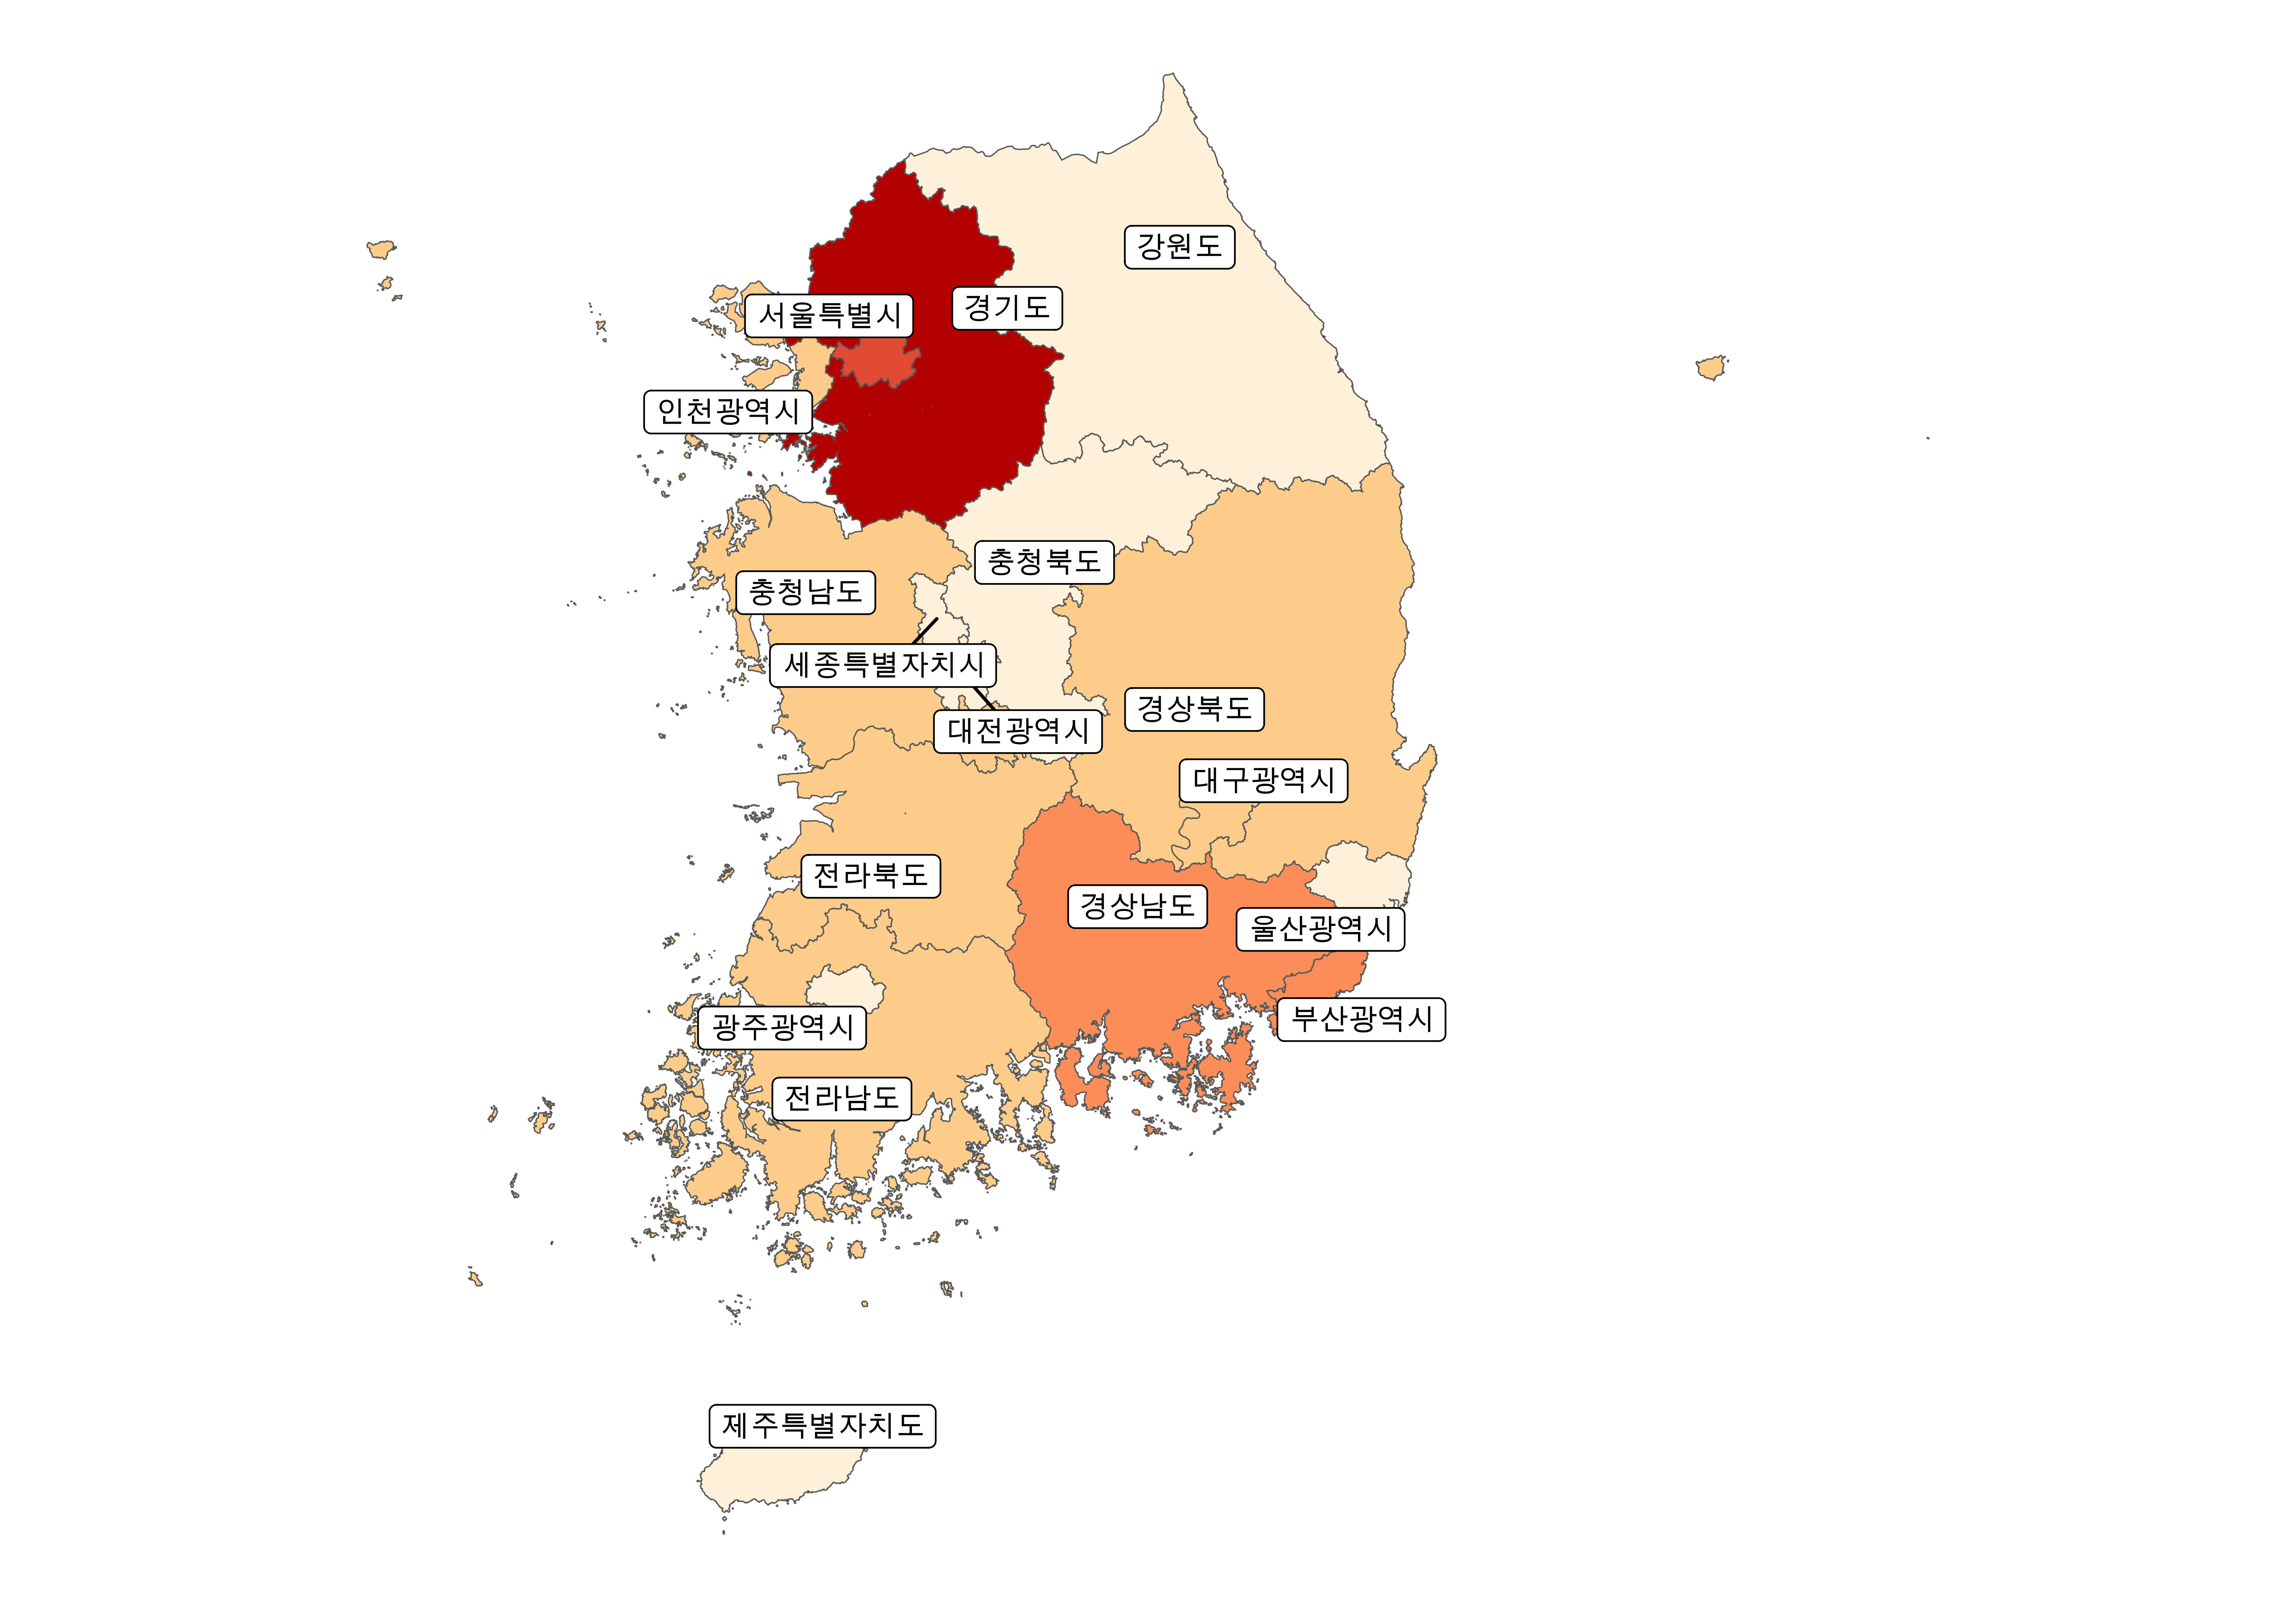
\includegraphics{images/GIS_tools.jpeg}

}

\caption{GIS 도구 활용 대한민국 시도별 인구수}

\end{figure}

\hypertarget{uxb9c8uxbb34uxb9ac}{%
\section{마무리}\label{uxb9c8uxbb34uxb9ac}}

공간정보 개발자와 사용자가 개발하는 코드는 기계보다 사람 친화적으로
바뀌었으며, 효과적인 디버그와 신속한 개발을 위한 파이프 철학도 도입되어
생산성 향상이 비약적으로 높아졌고 도구의 추상화 수준도 대폭 향상되었다.
IoT와 인공위성을 통해 엄청난 공간정보 데이터가 축적되고 있지만, GIS
도구가 꾸준히 발전하면서 이제 누구나 이러한 도구를 활용하여 공간정보
데이터를 통해 의미있는 산출물을 제작하고 도구도 개발할 수 있게 되었고,
다른 한편으로는 도구 없이 도구에 대한 이해없이 프롭테크를 논하는 것조차
의미없는 시대로 접어들고 있다.

\hypertarget{uxcc38uxace0uxbb38uxd5cc}{%
\section*{참고문헌}\label{uxcc38uxace0uxbb38uxd5cc}}
\addcontentsline{toc}{section}{참고문헌}

\printbibliography[heading=none]




\end{document}
